\chapter{Implementation}

In previous chapter, we designed a history system based of our previous analysis. Now we describe the actual implementation. 

We did not implement every part of the design because it is quite extensive. Instead, we chose parts of the design that bring the most value to users. Naturally, we also implemented parts of the design that are required for the system to actually work.

First, we identified the search application as the most important part of the design to implement. Second, we wanted to collect the usage of the shell history. To implement these two parts of the design, we needed to implement many other things. 

We need to integrate with the shell to collect history, context, and usage. Arrow key bindings are necessary to collect their usage. The search application also needed its custom key bindings. Daemon is necessary to process, save, load, and serve history data. Additionally, we also needed a convenient way to release the project and to deliver it to users.

\section{Shell integration}

In this section, we describe how our history system integrates into the shell so that is can provide the required functionality. 

\subsection{History collector}

Standard history does not contain context so we need to record it ourselves. 
We need to record contextual information both before and after the command line entry is executed. Most of the context is recorded before the execution but some context such as exit status is only available after the execution. 

We have two shell functions that record the context and send it to the daemon. One is called before and one after command line entry execution. In Zsh we used \verb|preexec| and \verb|precmd| hook functions to make Zsh call our functions at appropriate times. 

In Bash there are no native \verb|preexec| and \verb|precmd| hook functions. Luckily, there is a library \cite{lib-bash-preexec} that emulates these hook functions in Bash. The behavior is not always quite the same as in Zsh but we managed to work around all the issues we encountered with Bash.  

\subsection{Key bindings and line editing}

For many components of out history system we need a way to bind custom shell functions to keys so that they are launched when a key is pressed. Additionally, we often need to be able to manipulate the contents of the command line from these functions.

Zsh and Bash both have their own different built-in commands that allow us to bind shell functions to keys. Both shells also provide a different way to manipulate the command line contents. Ideally, we do not want to pollute our code base with many lines of shell specific code.

Unluckily, we could not find any library that provides a unified key bindings interface. Because of that, we created a library\cite{lib-bash-zsh-compat-widgets} that allows the same shell function to be bound to keys and used for command line editing in both Zsh and Bash. Additionally, the key bindings can be reverted to restore the original function.

% Bash issues and limitations 

% \subsection{Arrow key handler and collecting usage}

\section{Search application}

In this section, we describe the implementation of the notable parts of the search application. 

\subsection{Overview}

First, we look at the sequence of actions that happens when the search application is used. The sequence diagram in figure \ref{impl-search-app-sequence} shows the interactions of the user with different parts of the system.

At the start of the diagram the user presses \verb|CTRL-R| while on the shell prompt. Shell calls our custom shell function that wraps the search application. The shell function collects the current context and executes the search application; The context is passed using command line arguments. 


\begin{figure}
\centering
  \tmpframe{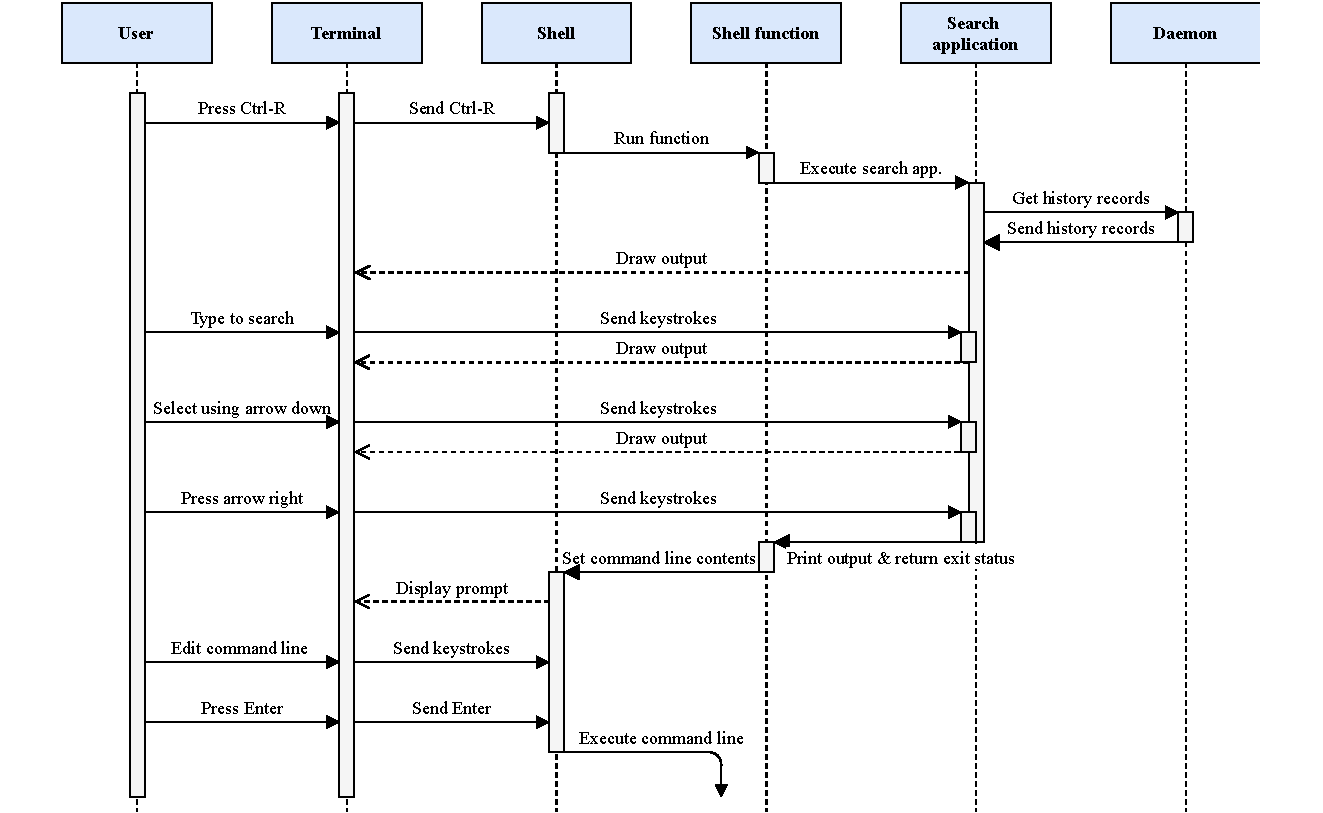
\includegraphics[angle=90,origin=c,width=\linewidth]{figures/implementation/thesis-impl-search-app-sequence-PADDING.pdf}}
  \caption{Sequence diagram of using the search application}
  \label{impl-search-app-sequence}
\end{figure}


The search application gets the history records from the daemon, searches the history, renders the results, and draws output to the terminal. We use a library\cite{lib-gocui} for creating terminal applications. This library takes care of drawing the output to the terminal and handling key bindings. Every time the user types something or presses any keys in the search application, the history is searched again and the results are rendered. 

When the user accepts the selected history entry, the application prints it to standard output and returns an exit status. 
The shell function captures the selected history entry; The history entry is written onto the command line. Based on the exit status, the shell function either executes the history entry or leaves it for the user to edit. The sequence diagram in figure \ref{impl-search-app-sequence} shows the latter. 

After the selected history entry is pasted onto the command line the user can further edit it. 
It is possible to use all standard editing capabilities of the shell to edit the command line.
Once the user accepts the command line the shell evaluates and executes it.




\subsection{Rendering}

In previous section, we covered how the search application interacts with the user and how it is launched from the shell. Now we describe the rendering process that happens inside the search application.


In figure \ref{impl-search-app-render-pipeline} we can see a schema of rendering pipeline. This pipeline is triggered as a response to any change in the search query made by the user. 


First, scores are calculated for all the history records. Then, the records are sorted by the score and filtered based on how many rows will fit in the terminal. After that, we render columns for history records that will be visible on the screen. At this point we determine how wide the individual columns should be. Finally, we put the columns together to render the full lines that will be displayed in the application.


\begin{figure}[h!]
\centering
  \tmpframe{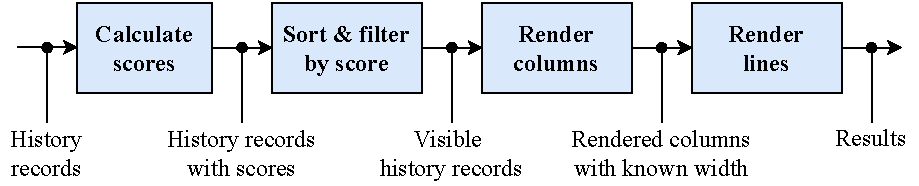
\includegraphics[width=\linewidth]{figures/implementation/thesis-ipml-rendering-pipeline.pdf}}
  \caption{Schema of rendering pipeline in the search application}
  \label{impl-search-app-render-pipeline}
\end{figure}



Now that we know how the rendering process works we can look at the screenshots from the search application. In the figure \ref{xterm-resh-normal-80}, we can see that the individual columns only take as much space as they need. 

The second screenshot in figure \ref{xterm-resh-normal-80-long} shows how the contents in the host and directory column are shortened. This happens when the contents are too long relative to the terminal width. The command line column takes up the rest of the terminal width. All shortened information for the selected result is displayed on the status line in full. 

In larger terminals a less compact time format is used; This is shown in figure \ref{xterm-resh-normal-full}.


\newpage
\begin{figure}
  \permanentframe{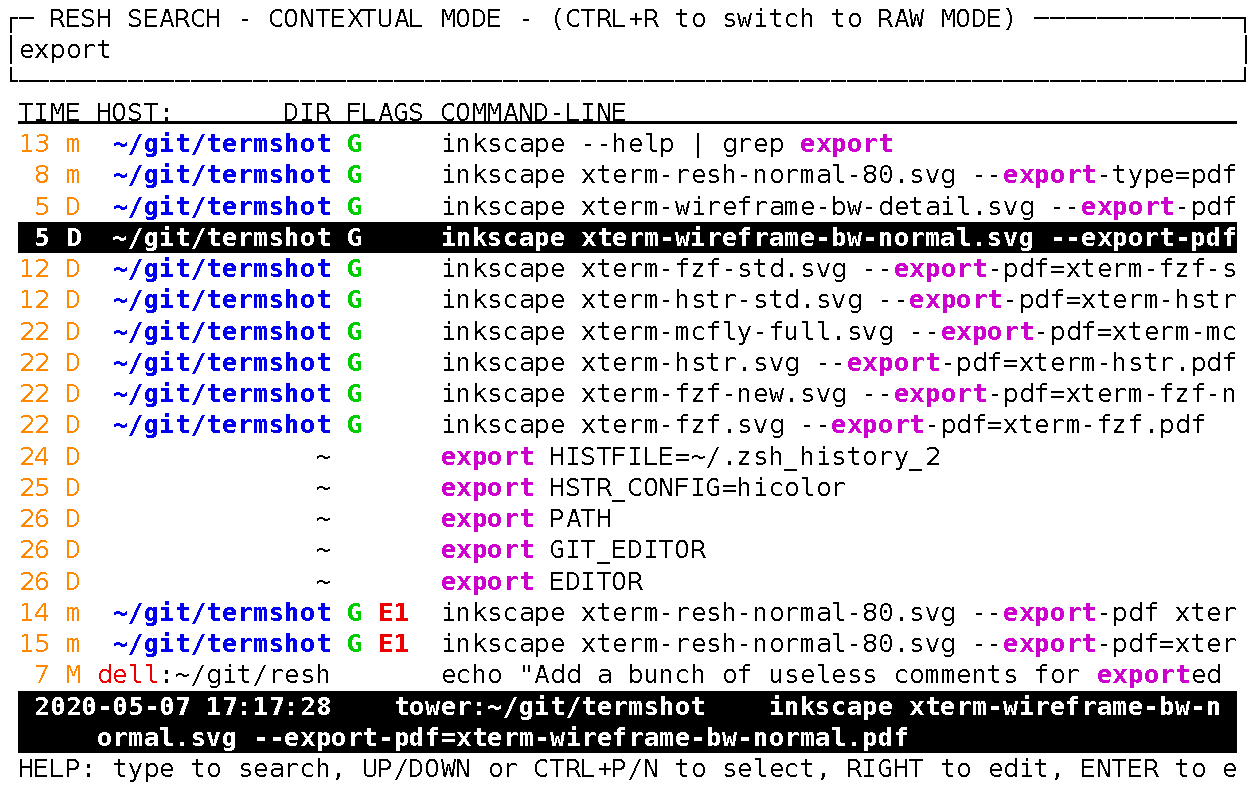
\includegraphics[width=0.995\linewidth]{figures/implementation/xterm-resh-normal-80.pdf}}
  \caption{Screenshot of the search application in the standard terminal size}
  \label{xterm-resh-normal-80}
\end{figure}

\begin{figure}
  \permanentframe{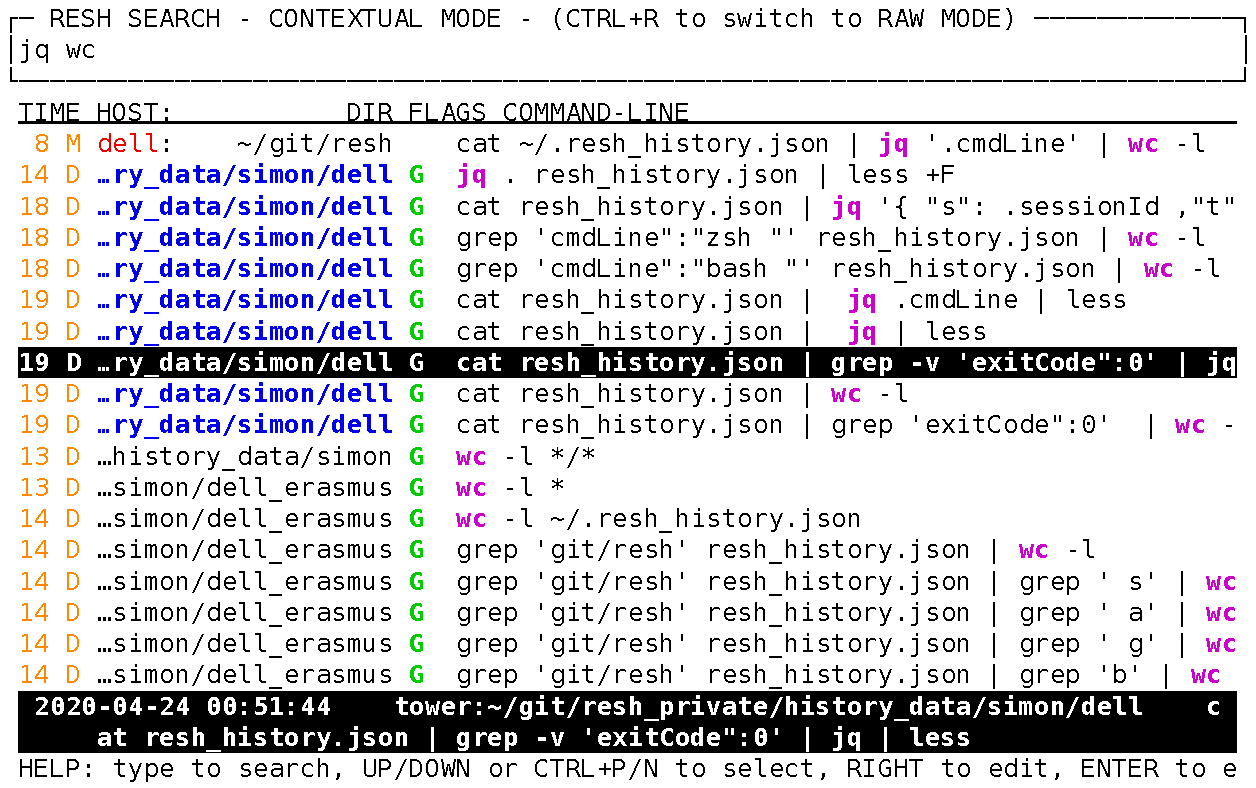
\includegraphics[width=0.995\linewidth]{figures/implementation/xterm-resh-normal-80-long.pdf}}
  \caption{Screenshot of the search application with wide columns}
  \label{xterm-resh-normal-80-long}
\end{figure}

\newpage
\begin{figure}
 \centering
  \permanentframe{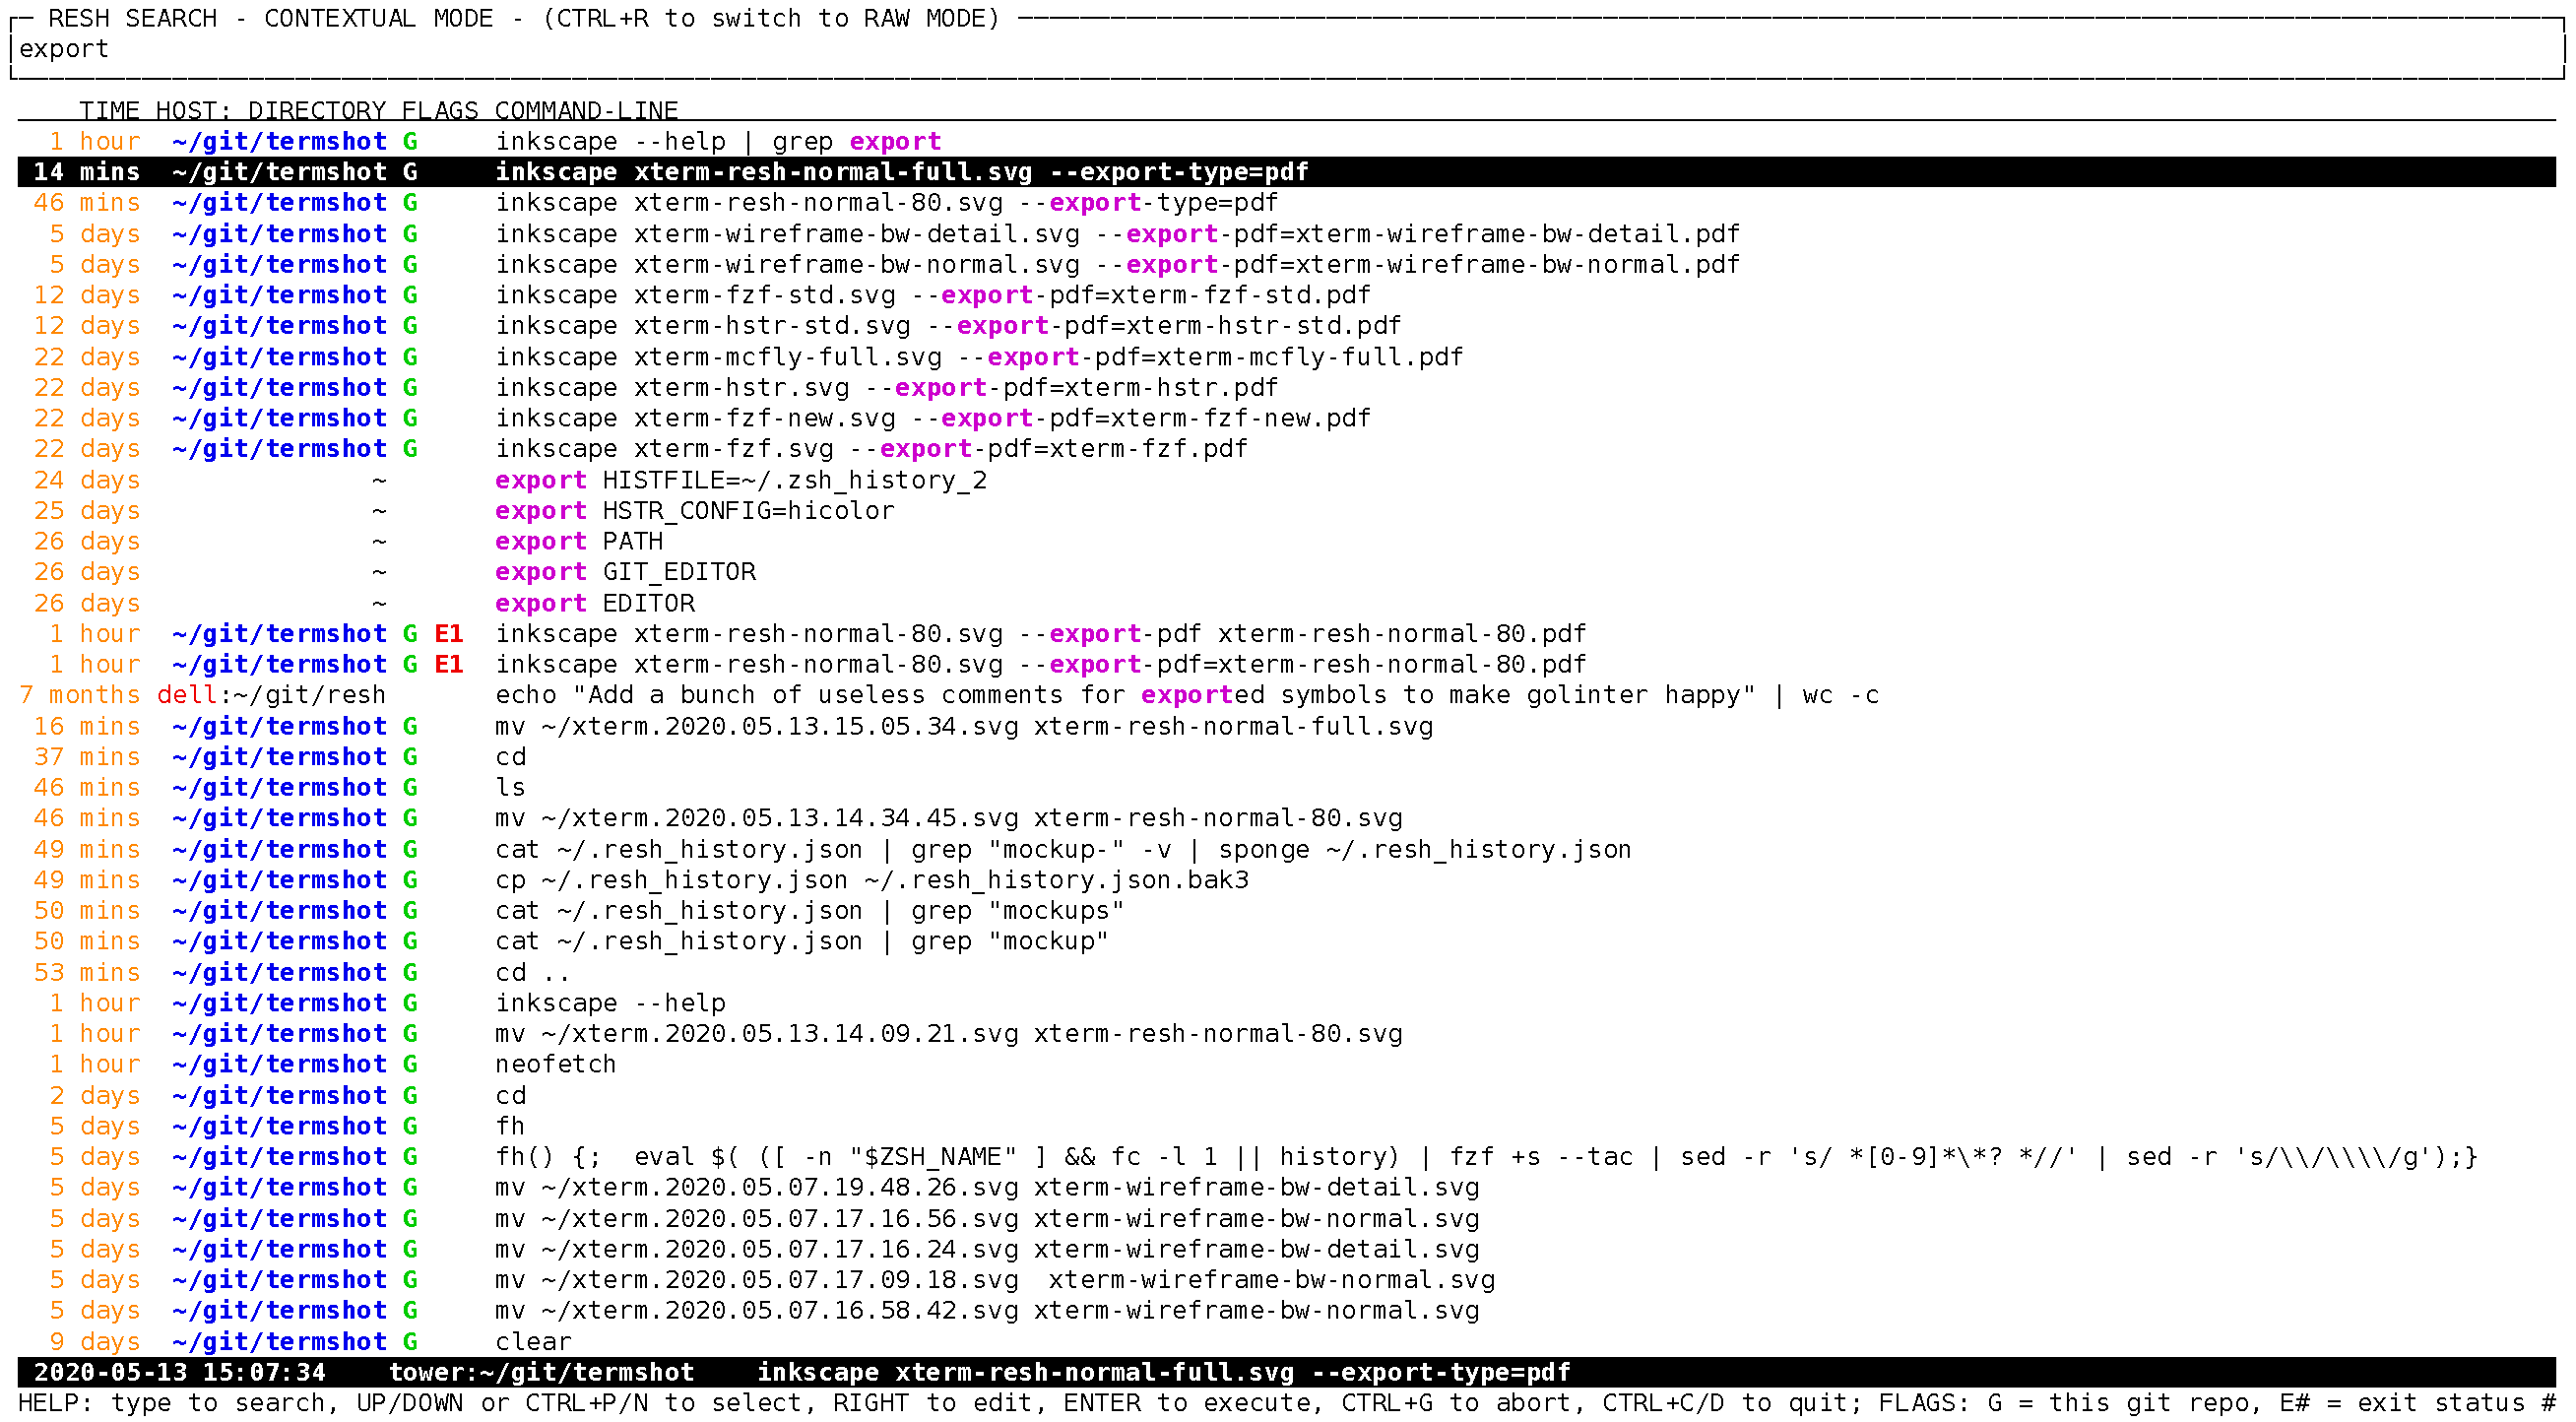
\includegraphics[angle=90,origin=c,width=0.87\linewidth]{figures/implementation/xterm-resh-normal-full.pdf}}
  \caption{Screenshot of the search application in a larger terminal}
  \label{xterm-resh-normal-full}
\end{figure}


\clearpage
\subsection{Calculating scores}

Earlier in figure \ref{impl-search-app-render-pipeline}, we saw calculating scores as one of the steps of the rendering process. Then we saw screenshots with search results which were searched and filtered based on scores. Now we describe how are the scores calculated.

As we explained earlier while designing, the scoring function consists of three partial scores:

\[ Score_r(q,c) = w_1 \cdot QueryScore_r(q) + w_2 \cdot ContextScore_r(c) + w_3 \cdot TimeScore_r \]


\paragraph{Query score}

To calculate the \(Query score\) we split the query into words by spaces. Then we take each word and we match it against the history entries. For each word of the query that matches the history entry the score is increased by \verb|1|. If the same word of the query matches multiple times we add \verb|0.002| to the score. 


We improve this simple matching algorithm by rewarding query words with extra score if they match whole commands or whole arguments. We implement this in a very naive way; Any string in the command line entry that is delimited by spaces is considered a separate "word". For each query word that matches any of these "words" we increase the score by \verb|0.33|.

\paragraph{Context score}

Earlier, we designed \(ContextScore\) to be calculated by comparing current context with the context of history records. This comparison should be based on four conditions shown in table \ref{tab:copy-of-score-matching-context}.

\begin{table}[h!]
\centering
\begin{tabular}{lll}
\hline \hline
Context condition       & Effect \\
\hline
Directory matches      & significantly increase score \\ 
Git repository matches & increase score \\ 
Non-zero exit status   & decrease score \\
Host does not match    & slightly decrease score \\ 
\hline \hline
\end{tabular}
\caption{Influence of different parts of context on \(ContextScore\) (table \ref{tab:score-matching-context})}
\label{tab:copy-of-score-matching-context}
\end{table}


There is an issue with these conditions; When directory matches it is almost certain that git repository matches as well. These conditions are highly correlated.
To fix that we introduce modified conditions as shown in table \ref{tab:score-context-impl-decorrelated}.

\begin{table}[h!]
\centering
\begin{tabular}{lll}
\hline \hline
Condition name & Description \\
\hline
DIR         & Directory matches \\ 
GIT         & Git remote matches AND Directory does not match\\ 
ERR         & Non-zero exit status \\
HOST        & Host does not match \\ 
\hline \hline
\end{tabular}
\caption{Decorrelated conditions of the \(ContextScore\)}
\label{tab:score-context-impl-decorrelated}
\end{table}

To determine scores for these conditions, we took at all possible combinations and we tried to ordered them. The order represents the desired behavior of \(ContextScore\); Any item in the list should get greater \(ContextScore\) than all items below it.


We found two useful ways to order the combinations. Other orders are either inconsistent or they do not match the importance of context conditions from table \ref{tab:copy-of-score-matching-context}. % For example, based on table \ref{tab:copy-of-score-matching-context}, \verb|DIR| has to be first and then we need to choose between \verb|GIT| and \verb|DIR \(\wedge\) HOST|. Once we make this choice we want to stick to it and 

\begin{multicols}{2}[]
Regular order:
\begin{itemize}
    \item DIR
    \item GIT
    \item DIR \(\wedge\) HOST
    \item GIT \(\wedge\) HOST
    \item DIR \(\wedge\) ERR
    \item GIT \(\wedge\) ERR
    \item DIR \(\wedge\) ERR \(\wedge\) HOST 
    \item GIT \(\wedge\) ERR \(\wedge\) HOST
    \item (no condition)
    \item HOST
    \item ERR
\end{itemize}

Order with reduced penalty for non-matching host:
\begin{itemize}
    \item DIR
    \item DIR \(\wedge\) HOST
    \item GIT
    \item GIT \(\wedge\) HOST
    \item DIR \(\wedge\) ERR
    \item DIR \(\wedge\) ERR \(\wedge\) HOST
    \item GIT \(\wedge\) ERR
    \item GIT \(\wedge\) ERR \(\wedge\) HOST
    \item (no condition)
    \item HOST
    \item ERR
\end{itemize}
\end{multicols}

Out of these two orders we decided to use the "Regular order". This order should be better at handling situations where there are many different hosts with a lot of history. According to our previous design, each combination of conditions should result in a unique \(ContextScore\). Table \ref{tab:score-context-impl-values} shows how we assigned scores to the individual conditions in a way that produces unique result for each combination of conditions.

\begin{table}[h!]
\centering
\begin{tabular}{lr}
\hline \hline
Condition name & Score \\
\hline
DIR         & \(0.9\)   \\ 
GIT         & \(0.8\)   \\ 
ERR         & \(-0.4\)     \\
HOST        & \(-0.2\)     \\ 
\hline \hline
\end{tabular}
\caption{Scores for conditions of \(ContextScore\)}
\label{tab:score-context-impl-values}
\end{table}

\paragraph{Time score}


To calculate the \(TimeScore\) we take the number of seconds since epoch and we multiply them by a coefficient to scale them to a number lower than one. The specific constant we use is $1\mathrm{e}{-10}$.

\paragraph{Score weights}

Now that we covered how we implement the partial scores we need to combine them together.
First we want to make sure that the user can search effectively. We do not want to show results with matching context before these that match the search query. This means that a single match of a query should result in a \(QueryScore\) greater than any \(ContextScore\).

Formally, for a single word query \(q\) that matches record \(r\), for all contexts, and for all records following should hold: 

\[  w_1 \cdot QueryScore_r(q) > \max{(w_2 \cdot ContextScore)} \]

Furthermore, we do not want the contextual penalty to hide history results that match the query. We extend the previous rule to include this; For a single word query \(q\) that matches record \(r\), for all contexts, and for all records following should hold:

\[  w_1 \cdot QueryScore_r(q) + \min{(w_2 \cdot ContextScore_r)} > \max{(w_2 \cdot ContextScore)} \]

When we set \(w_2\) to \(1\) and fill in values based on definitions of the partial scores we get:

\[  w_1 \cdot 1 - 0.6 > 0.9 \]

For \(ContextScore\) weight equal to \(1\), the weight for \(QueryScore\) (\(w_1\)) needs to be greater than \(1.5\). This way a single query match has enough influence compared to the context.

Now we have determined all weights except for \(TimeScore\) weight. We only want \(TimeScore\) to influence the order when everything else is equivalent. To do this we set the weigth for \(TimeScore\) (\(w_3\)) to $1\mathrm{e}{-3}$.

% final weigths 1.51, 1, 1e-3

\section{Daemon}

So far we covered the implementation of the search application and the necessary shell integration. Now we describe how we implement the daemon.

%\subsection{Overview}

As you can see in figure \ref{impl-daemon-channels}, the daemon consists of four parts that communicate asynchronously using Go channels\cite{lib-go-channels}. We use standard Go http server\cite{lib-go-http} to listen for requests. 

The history collector uses \verb|/record| request to send history records to the daemon. The search application uses \verb|/dump| request to get all history records. And the \verb|/recall| request is used by the arrow key handler to get a command line entries from the daemon. 

All of the requests use JSON as a data exchange format. Conveniently, history records are also saved to storage as JSON.

\begin{figure}
\centering
  \tmpframe{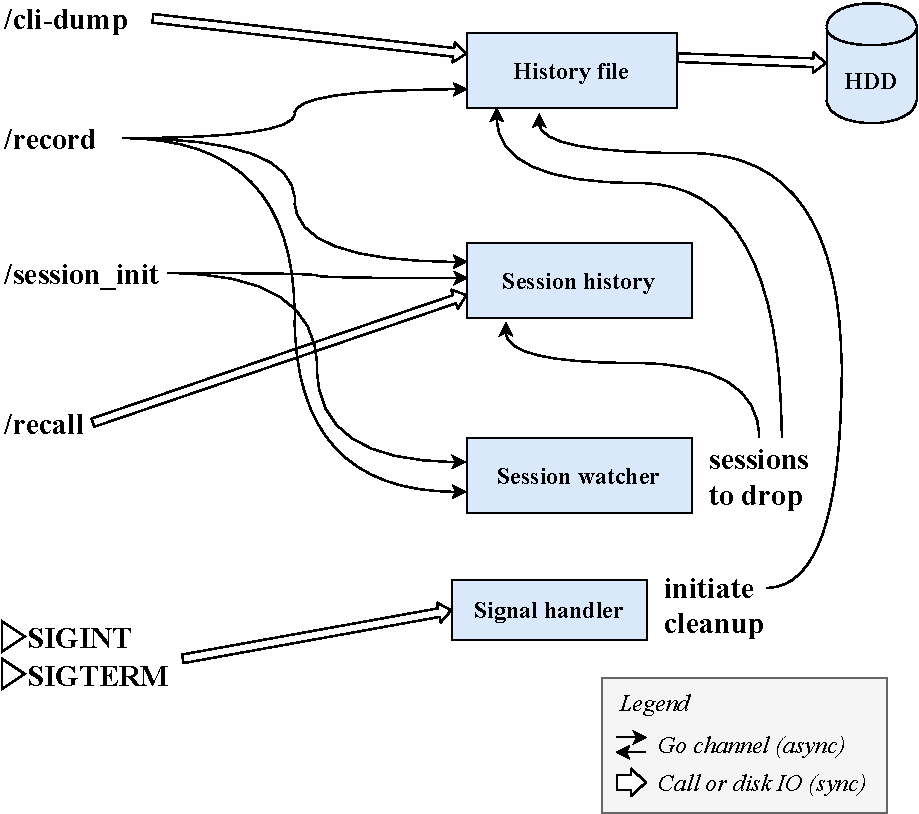
\includegraphics[width=\linewidth]{figures/implementation/thesis-impl-daemon-channels.pdf}}
  \caption{Schema of internal daemon structure and communication}
  \label{impl-daemon-channels}
\end{figure}

\subsection{History file}

The history file module is responsible of all communication with storage device. It reads history records from storage when it starts up. And it also writes history records to storage.

Earlier, we explained that history collector is activated before and after each executed command line. This means that the history record is sent to the daemon in two parts. The history file module is responsible for merging the two parts into a single history record. 

When the search application sends \verb|/dump| request the history file module responds with all history records. 

% standard shell history

\subsection{Session history}

The session history module holds history for active sessions. It receives history records from \verb|/record| requests and appends them to history for matching session.
These session history structures only exist in memory.

The session history module responds to \verb|/recall| requests from the arrow key handler. The history for the session is retrieved and an appropriate history entry is returned. 

\subsection{Session watcher}

The session watcher module is responsible for keeping track of which sessions are no longer active. Any history records sent to the daemon using \verb|/record| requests are also sent to the session watcher module. 

Whenever a new history record is received the session watched module looks at the session it belongs to. If it is not already watching this session it starts periodically checking if the session is still active. Specifically, we check if the process with the PID of the session is still running.

Once a session becomes inactive, the session watcher module notifies the session history and the history file modules. These modules delete appropriate structures from memory.

\subsection{Signal handler}

The signal handler module is responsible for shutting down the daemon when it receives \verb|SIGINT| or \verb|SIGTERM| signal. First, it notifies the history file module to write out all pending history records to the storage device. Once this is done or a timeout is exceeded the signal handler module shuts down the whole daemon.


\section{Installation, updates, and configuration}

Writing the software is just the first part of the process. Releasing it and getting it to your users is equally important. In this section, we describe how we build the project and how users can install it.

\subsection{Releasing and building the project}

Our project is hosted on GitHub\cite{resh-github-homepage}. We have setup a CI pipline to build binaries of the project for every tag we push to the repository. Specifically, we use GitHub Actions\cite{github-actions} and Goreleaser\cite{tools-goreleaser}.

When the CI pipeline builds the binaries it creates a new release on the release page\cite{resh-github-releases}. The built binaries are available there. 

\subsection{Installation and updates}

The project can be installed by running a single command:

\begin{verbatim}
curl -fsSL https://raw.githubusercontent.com/curusarn/resh
    /master/scripts/rawinstall.sh | bash
\end{verbatim}

First, the script checks the operating system and the CPU architecture of the device. Based on that an archive with appropriate binaries is downloaded. Then, an integrity check is performed and the archive is extracted. 

After extracting the archive, we check versions of Bash and Zsh, make directories, and copy files. We also append a few lines to users dotfiles to setup the shell integration. Finally, we show some onboarding information to the user.

The project has almost no dependencies; There are only a very standard utilities required for installation. The binaries are statically linked so they do not depend on any system libraries.

The project can be updated at any time by running \verb|reshctl update|. This checks if there is a new version of the project available and installs it.

\subsection{Configuration and control}

Our project comes with a configuration command \verb|reshctl|. Basides other things, this command can be used to enable and disable key bindings. 

Tab completions for \verb|reshctl| are set up during installation. There is a help (\verb|-h|/\verb|--help|) option available with descriptions for individual subcommands. To make it easy to provide all this, we use a library\cite{lib-go-cobra} for creating command line interfaces.
